\AntoineSpeak	
\subsection{Github  et travail collaboratif}	% A Florent
\begin{frame}{Github, plateforme de travail collaboratif} % A.  
	\begin{itemize}
		\item Communication et versionnement
		\begin{figure}
			\centering
			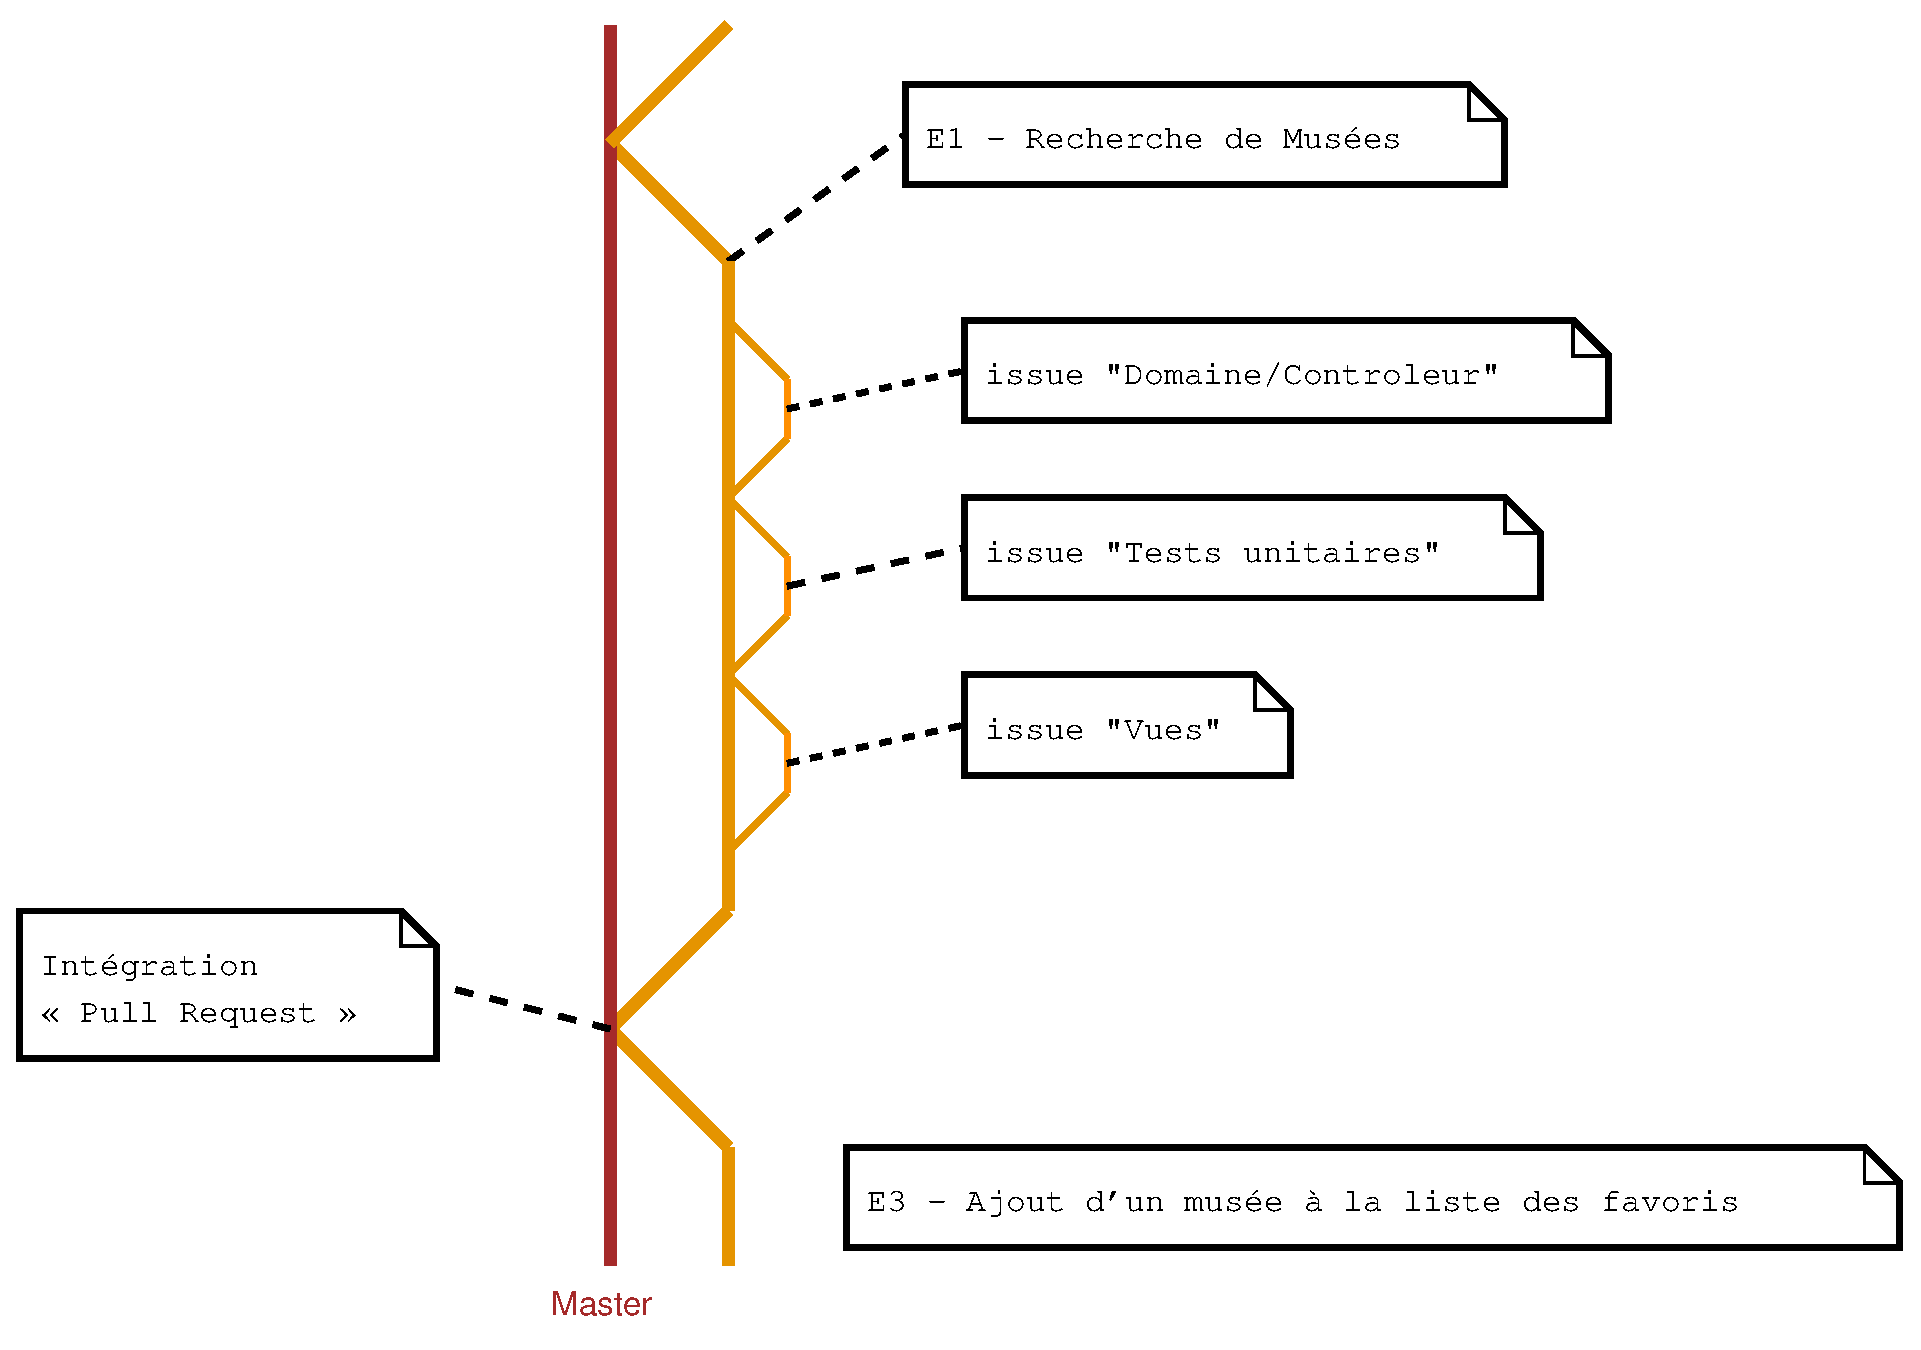
\includegraphics[width=9cm]{./images/workflow_github}
			\caption{Workflow sur GitHub}
			\label{fig:workflow_github}
		\end{figure}
	\end{itemize}
\end{frame}

\begin{frame}{Github, plateforme de travail collaboratif} % A.
	\begin{block}{Une exigence est terminée, si}
		\begin{itemize}
			\item Le code est \textbf{lisible} et \textbf{compréhensible}
			\item Le code est correctement \textbf{documenté}
			\item Les \textbf{tests} passent \cmark
		\end{itemize} 
	\end{block}
	\pause

	\begin{block}{Utilisation des Pull Requests}
		\begin{itemize}
			\item Création par la personne s'affectant l'issue
			\item Description du travail accompli
			\item PR validée par un autre membre de l'équipe
				\begin{itemize}
					\item Respect de la définition de \textbf{<< finie >>}
					\item \textbf{Tests fonctionnels} \cmark
				\end{itemize}
		\end{itemize}
	\end{block}
\end{frame}

